\section{Same side track identification using a Boosted Decision Tree}
\label{sec:SS_classifier}

To identify tracks that belong to the SS of a signal~$B$, a BDT is trained on the simulated LHCb data. 
The BDT output resembles an estimated probability of the track being in the SS and is from now on called $\text{Prob}_\text{SS}$.
The implementation of the BDT is done with the library \textsc{XGBoost} \cite{xgboost}.

The dataset used for training the BDT contains about 70 different features of the tracks of the associated event.
To reduce this list of features, first the correlation coefficient between all feature pairs is calculated.
Features with a correlation near $100\%$ are considered to contain redundant information.
Only one feature of each set of highly correlated features is kept for training the BDT.
Next, a BDT is trained on a dataset containing all features and the gain of each feature is calculated.
The gain is a measure used in decision trees to estimate the accuracy improvement of the introduction of a cut on one feature.
Additionally, the permutation importance of the ROC AUC is calculated.
The permutation importance is the difference in any performance metric after making predictions on a dataset with the entries of a single feature permuted at random.
The features with the lowest gain or permutation importance are discarded until a reasonable amount of features is achieved.
The remaining 21 features are listed in \cref{tab:SS_features} together with the corresponding feature importances shown in \cref{fig:SS_importances}.

\begin{figure}
    \centering
    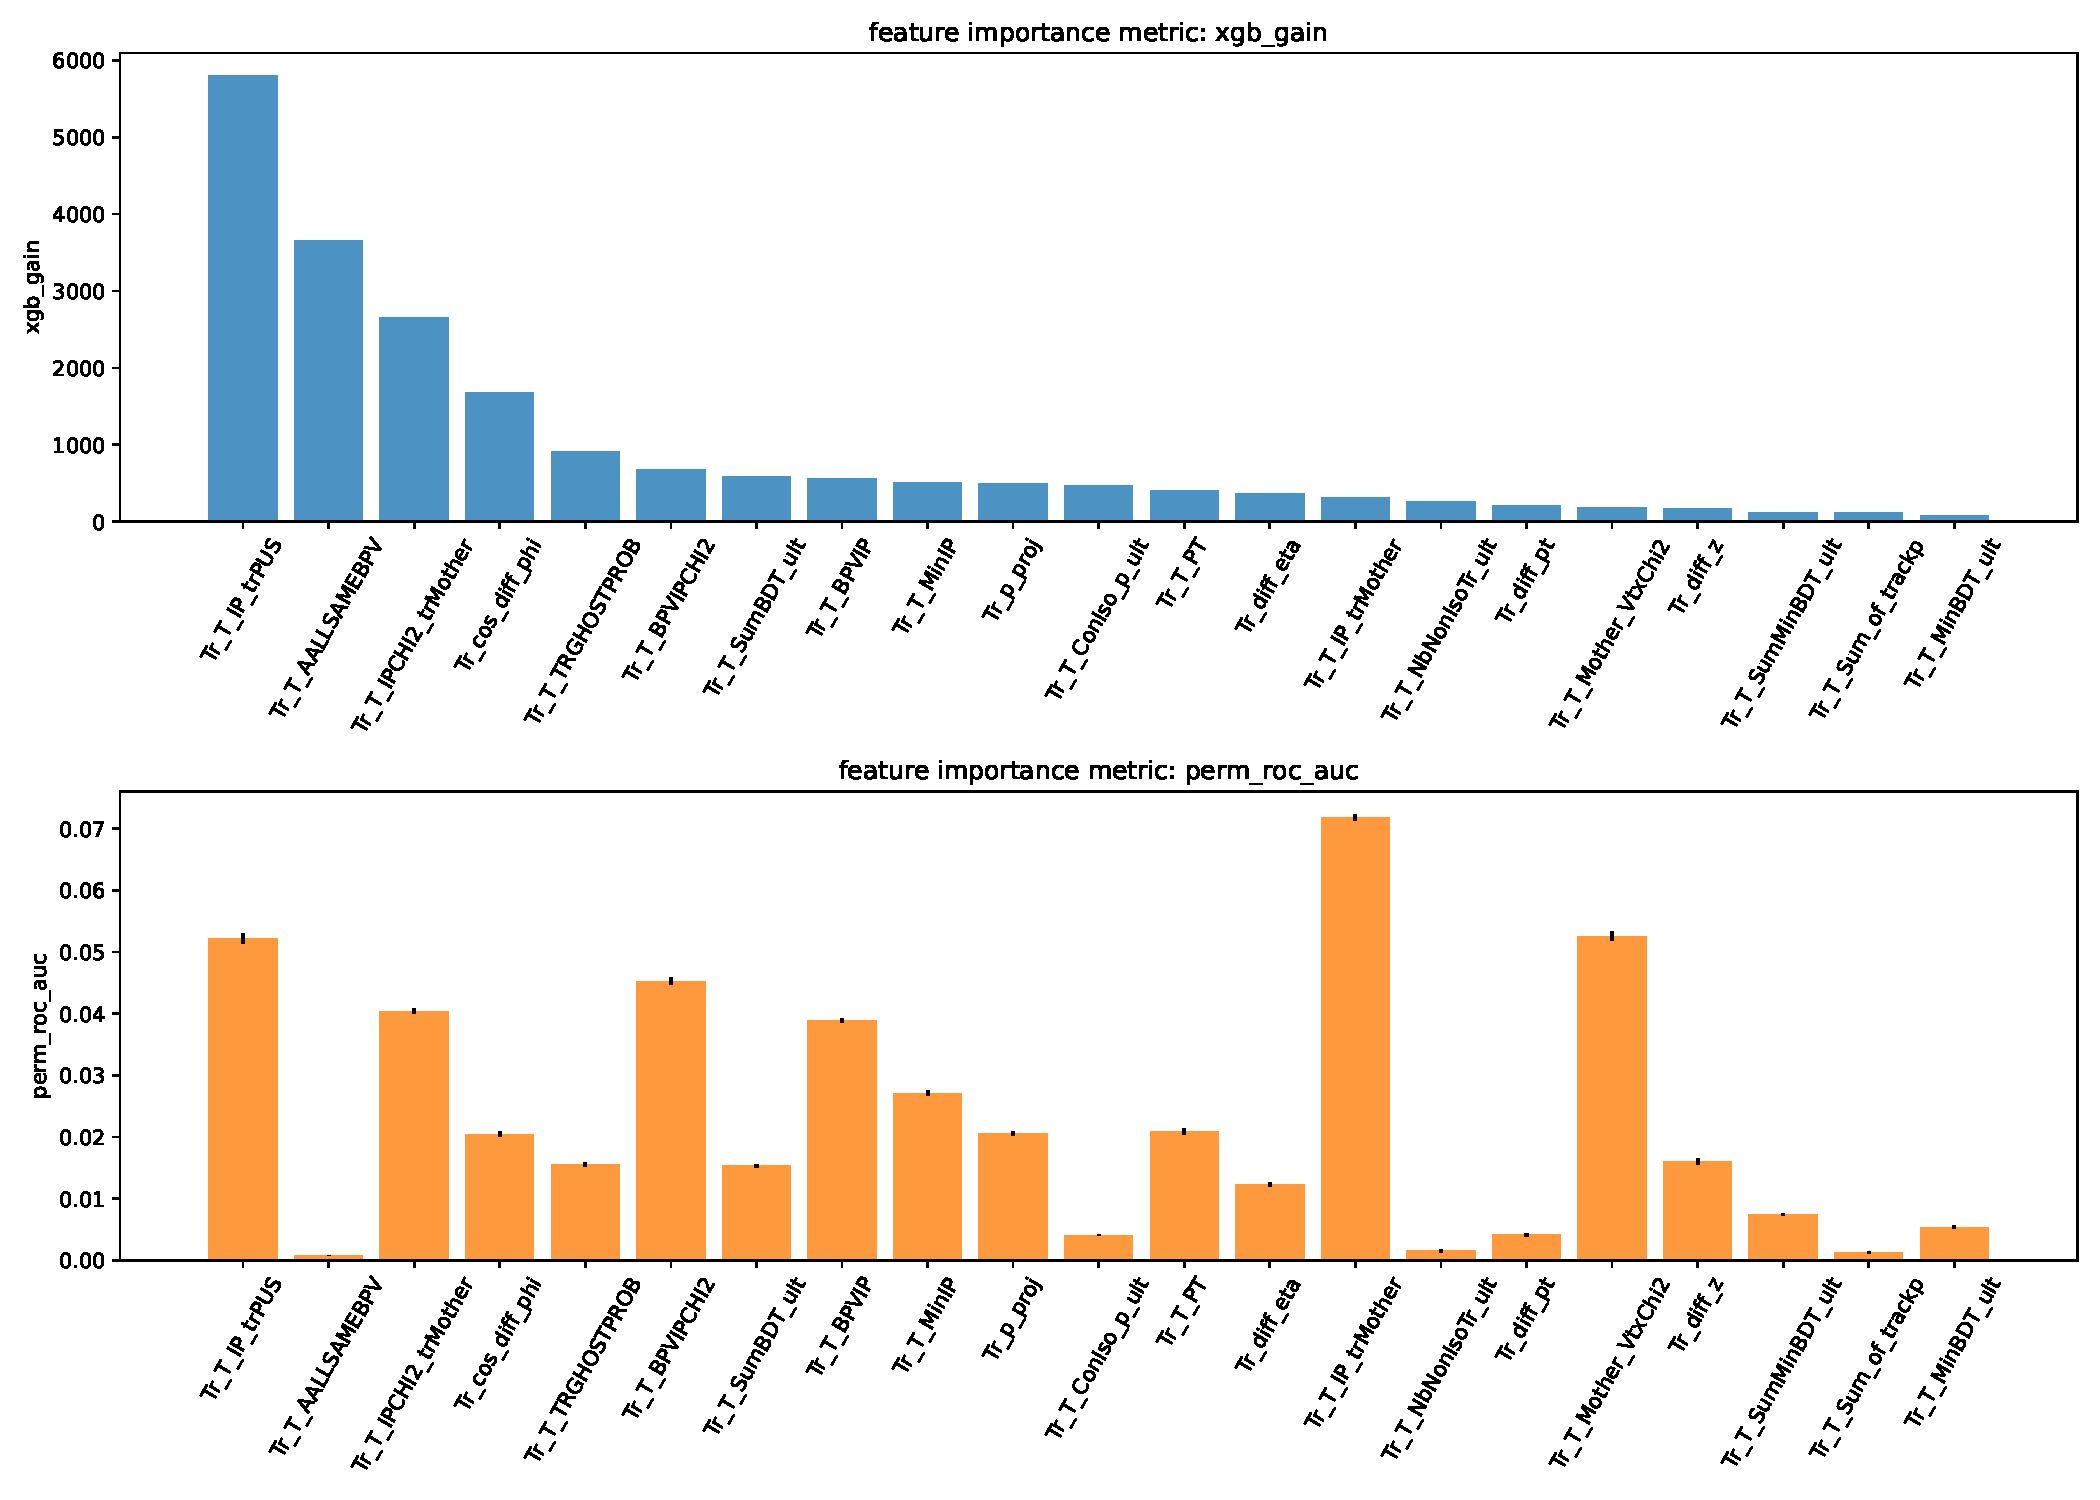
\includegraphics[width=\textwidth]{images/SS_feature_importances.pdf}
    \caption{Calculated feature importances on the trained BDT for SS track identification. Shown are the gains and the permutation importances of the ROC AUC normed on the largest value.}
    \label{fig:SS_importances}
\end{figure}

\begin{table}
    \centering
    \caption{List of all features used to train the BDT for SS track identification.}
    \label{tab:SS_features}
    \begin{tabular}{c c}
        \toprule
        feature & feature \\
        \midrule
        $p_\text{T}$        & $\text{IP}_\text{SV}$ \\ 
        $p_\text{proj}$     & $\chi^2(\text{IP}_\text{SV})$ \\ 
        $\Delta p_\text{T}$ & $\sigma(\text{IP}_\text{pileup vtx})$ \\ 
        $\Delta z$          & $\text{IP}_\text{best PV}$ \\    
        $\Delta \eta$       & $\chi^2(\text{IP}_\text{best PV})$ \\ 
        $\cos(\Delta \phi)$ & $\text{IP}_\text{min}$ \\ 
        $\text{Prob}_\text{ghost}$ & same PV \\
        $\chi^2(\text{vtx})$     & cone isolation \\
        SumBDT              & $N_\text{non iso}$ \\ 
        MinBDT              & $\sum p_\text{in cone}$ \\ 
        SumMinBDT           &  \\
        \bottomrule
    \end{tabular}
\end{table}

%(Explain all features)....
All the following features describe a single particle or rather its reconstructed track.
%
The transversal momentum is denoted by $p_\text{T}$. 
%
Some features are also defined for relation between the signal $B$ and the reconstructed track. 
$p_\text{proj}$ is the dot product of the 4-momenta,
$\Delta p_\text{T}$ is the difference of the transversal momenta,    
$\Delta \eta$ is the difference of the pseudorapidities and   
$\cos(\Delta \phi)$ is the cosine of the difference of the $\phi$-coordinates. 
$\Delta z$ is the $z$-coordinate difference of the PV and the first detector hit of the track. 
%  
$\text{Prob}_\text{ghost}$ is an estimated probability that the track is falsely reconstructed and does not belong to an actual particle. 
$\chi^2(\text{vtx})$ is the $\chi^2$ of the combined reconstructed vertex of the signal~$B$ and the track. 
\enquote{same PV} refers to whether the particle's vertex is the same as the PV.
%
An impact parameter (IP) is the minimum distance of a track to a given point.
$\text{IP}_\text{SV}$ is the IP to the SV and  
$\chi^2(\text{IP}_\text{SV})$ is its uncertainty.
$\sigma(\text{IP}_\text{pileup vtx})$ is the significance of the IP to the closest pileup vertex,
$\text{IP}_\text{best PV}$ is the IP to the best estimated PV and  
$\chi^2(\text{IP}_\text{best PV})$ is its uncertainty.
$\text{IP}_\text{min}$ is the minimum IP with respect to all PV candidates.
%
Cone-isolation refers to an isolation metric of a track which is evaluated based on how many neighbouring tracks are inside a defined cone in the $\eta$-$\phi$-plane around the track in question.
SumBDT,    
MinBDT and    
SumMinBDT describe the cone-isolation based on multiple BDT classifiers which work on the mentioned principle.
$\sum p_\text{in cone}$ is the sum of the absolute momenta of all particle tracks in the defined cone.
The feature \enquote{cone isolation} describes the momentum based cone-isolation $p/\sum p_\text{in cone}$. 
$N_\text{non iso}$ is the number of tracks not isolated from the track.   

Then a BDT is trained on a dataset containing all features of this list.
From the $18$ million tracks in the dataset, $60\%$ are used for training and $40\%$ are used for validation of the trained model.
The trained model contains $2000$ estimators at a maximum decision tree depth of $4$.
The learning rate is set to $0.1$.
Due to the imbalance of SS tracks and other tracks in the data ($N_\text{SS}/N_\text{other} \approx 0.084$), a parameter that controls the balance of positive and negative weights of the BDT is set accordingly. 
The learning objective is logistic regression for binary classification.

The negative log-likelihood and the error rate for each iteration of the training of the BDT are shown in \cref{fig:SS_history}.
The error rate is the proportion of predictions matching the true labels of the simulation.
For this, all tracks with $\text{Prob}_\text{SS}>0.5$ count as predicted SS tracks. 

\begin{figure}
    \centering
    \begin{subfigure}{0.5\textwidth}
        \centering
        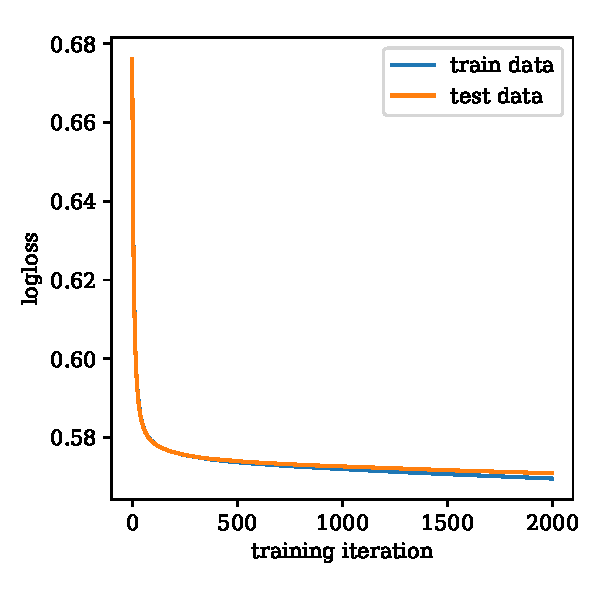
\includegraphics[width=\textwidth]{images/SS_history_logloss.pdf}
        \caption{Negative log-likelihood during training}
    \end{subfigure}%
    \begin{subfigure}{0.5\textwidth}
        \centering
        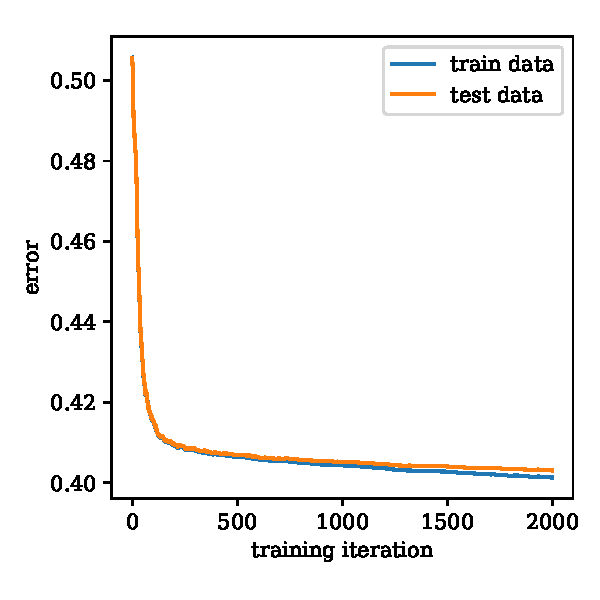
\includegraphics[width=\textwidth]{images/SS_history_error.pdf}
        \caption{Error rate during training}
    \end{subfigure}%
    \caption{Performance of the BDT for SS track identification after each training iteration.}
    \label{fig:SS_history}
\end{figure}

To show the achieved separation of the SS tracks, histograms of $\text{Prob}_\text{SS}$ split by the true labels of the simulation are shown in \cref{fig:SS_output}.
A measure of separation is the ROC (reciever operating characteristic) curve shown in \cref{fig:SS_ROC}.
To estimate the generalization and overtraining of the model, each performance measure is calculated on both the test data and training data.
The achieved ROC AUC (area under the ROC curve) is $0.763$ on the test data and $0.767$ on the training data.
A ROC AUC of $1.0$ means perfect separation and a ROC AUC of $0.5$ means no separation.

\begin{figure}
    \centering
    \begin{subfigure}{0.5\textwidth}
        \centering
        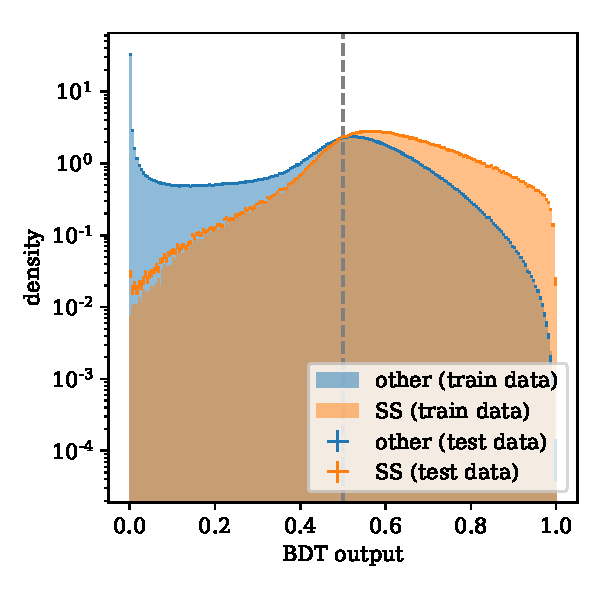
\includegraphics[width=\textwidth]{images/SS_output.pdf}
        \caption{Distribution of $\text{Prob}_\text{SS}$}
        \label{fig:SS_output}
    \end{subfigure}%
    \begin{subfigure}{0.5\textwidth}
        \centering
        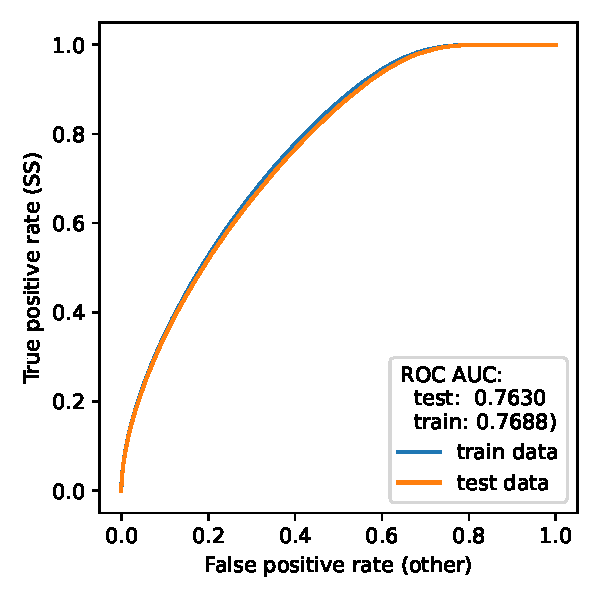
\includegraphics[width=\textwidth]{images/SS_ROC.pdf}
        \caption{ROC curve of the BDT predictions}
        \label{fig:SS_ROC}
    \end{subfigure}%
    \caption{The left figure shows the distribution of the BDT output split by the true labels of the simulation. The right figure shows the ROC curve of the BDT output. Both figures show the BDT prediction for the test data and the training data.}
    \label{fig:SS_eval}
\end{figure}
